\chapter{Open Microfluidics}\footnote{This chapter has been modified from the manuscript in preparation of the same title. The manuscript includes as authors Erwin Berthier, Theodorus de Groot, Jean Berthier, Benjamin Casavant, and David Beebe}
\label{Chap:OpenMicrofluidics}


\section{Introduction}
Microfluidic systems are fundamentally transforming medicine, diagnostics, and analytical systems, at an academic and industry level. In particular, microfluidics enables a more efficient use of rare samples and reagents \cite{Burns1998, Ingham2007, Song2006a, Thorsen2002a}, observations and measurements at single molecule or cell levels \cite{Kopp1998, Hong2012}, and engineering platforms of higher relevance to the system being studied \cite{Berthier2013,Huh2010a,Jeon2015,Meyvantsson2008,Sackmann2014a,Domenech2009}. Despite enabling features, microfluidics come with significant challenges that pose barriers to adoption. Manufacturing enclosed channels at a sub-millimetric scale is a ubiquitous step in traditional microfluidic platforms that increases cost and complexity of fabrication \cite{Guckenberger2015b,Sackmann2014}. At the industry level, this step often involves highly-guarded trade secrets that slow innovation and development of microfluidic-based products. Usability, reliability, and accessibility are also renown difficulties that limit the field of use and audience for microdevices \cite{Casavant2013, Sackmann2014}. Here, we present advances in open microfluidics, a novel approach to designing microfluidic systems that allows the precision of traditional closed microfluidic systems while fundamentally improving affordability, simplicity, and reliability.

The development of simple methods that lower the barriers of adoption for microfluidic systems has increasingly been a focus of research \cite{Berthier2013,Casavant2013b, Du2009, Guckenberger2015, Walker2002, Young2011}. Seminal innovations in microfluidic technologies have proven that a reduction in the complexity of use or fabrication result in an exponential growth in the adoption of these systems \cite{Berthier2012,Sackmann2014a}. The initial widely recognized development in microfabrication that unlocked the field for widespread adoption is soft lithography and the use of silicone polymers for device fabrication \cite{Sia2003a}. Other developments of importance to medicine and diagnostics that expanded the breadth of applications was the use of thermoplastics through micromilling \cite{Guckenberger2015b, Wilson2011}, hot-embossing \cite{Young2011}, or laser cutting \cite{Klank2002, Yuen2009MultidimensionalSystem}. The emergence of high-resolution stereolithography additive printing (SLA, a form of 3D printing) is promising to rapidly transform the field of microfluidics. In particular, 3D-printing facilitates the design-to-manufacturing transition and microfluidic assembly, as it enables the production of ready-to-use channels that do not require bonding or other forms of preparation \cite{Au2014, Bhargava2014}. However, SLA imposes important material limitations (e.g. limited biocompatibility) and uncured resin must be removed from the channels after manufacturing thereby limiting the complexity of the geometries achievable. Simplification of microfluidics technologies has also been demonstrated by using paper fibers as both a path for fluid and a pumping method, showing great promise to develop ultra-low cost diagnostic and detection systems \cite{Martinez2008, Osborn2010a, Park2013a}. Paper-based devices are incredibly cost-effective to produce, user-friendly and intuitive to operate, and reliable to use since they don’t rely on pressure sources, seals, and cannot fail due to air bubbles. However fluid handling in paper is limited, in particular the ability to exchange and wash fluids, and material interaction and adsorption challenges are increased due to the high surface-to-volume ratios. The common theme of microfluidic development is the reduction of manufacturing and user-operation cost and complexity. There remains, however, a trade-off between control over the fluid and operational simplicity.

Open microfluidics describes the flow of fluids in channels that have one or more open faces; the simplest being a rectangular channel with no ceiling \cite{Berthier2012, Casavant2013}. Open microfluidics allows the control over fluids on-par with traditional closed-fluidics while providing manufacturing simplicity and reliability of use on par with paper-microfluidics. In open microfluidics, fluid flow is driven directed by capillary force provided by the solid parts of the cross section of the channel allowing the fluid to span over the open sections of the cross section. We compile here the initial forays of open microfluidics and expand on them to demonstrate the potential of open microfluidics to further democratize the prototyping and manufacturing of microfluidic-based systems that are reliable and low-cost. We show that open microfluidics is a ubiquitous technology that enables control over fluid handling, access to the sample throughout the device operation, simple manufacturing and prototyping (compatible with injection molding and 3D printing), and the potential to create non-planar reconfigurable systems. We present a suite of devices that are driven by open microfluidics and designed to overcome many limitations that current microfluidic platforms have to adoption research communities at large. Finally, we show that reconfigurable systems can be created utilizing the example of Lego-like blocks that enable the creation of a bread-board microfluidic system that can be modified during the operation of the device.

\section{Results and discussion}

\subsection{Open microfluidic conditions for flow}
Open microfluidics is a class of microfluidic channels that are defined as having one or more open-air interfaces along the path of the channels (Figure \ref{figure:OpenFig1}A). Early work has developed an analytical model that allows the design of open microfluidic systems in which capillary flow occurs, termed spontaneous capillary flow (SCF) \cite{Casavant2013}. Subsequent analytical and numerical simulation-based work have demonstrated an improved equation to predict the flow in open systems based on any number of surfaces each with a distinct surface energy (resulting in an apparent contact angle for the whole system, known as the generalized Cassie’s law [ref], Figure \ref{figure:OpenFig1}B). Experimentally, open microfluidic systems have demonstrated the potential to create enabling systems for analytical chemistry (liquid-liquid extractions)\cite{Barkal2016}, and cell biology (cell migration) that are highly accessible and manufacturable. For increased connectivity flows can be designed with no ceiling or floor in which the fluid is simply pinned from both edges (Figure \ref{figure:OpenFig1}A). These types of flows allow the addition of dual stimuli to the channel. For increased capillary force, as detailed in the flow conditions presented in figure 1, flows can be designed using parallel beams or fibers (Figure \ref{figure:OpenFig1}A).

The conditions for flow to occur in bulk (i.e. not as individual Concus-Finn filaments in wedges) in an open microfluidic channel have been demonstrated \cite{Casavant2013} and are summarized in figure 1B. For a material with a contact angle , a length of   along the cross-sectional perimeter representing the liquid-solid interfaces, and a length of  along the cross-sectional perimeter representing the liquid-air interfaces, the conditions for flow are described by equation \ref{equation:OpenEq1}. When this condition is met fluid flow occurs by capillary action in the microfluidic network and functional systems can be developed. Else capillary flow as a bulk in the channel does not occur. 

\begin{equation}
    cos\ \theta> \frac{P_f}{P_w}
    \label{equation:OpenEq1}
\end{equation}

The conditions for flow has been generalized for an open channel that is composed of any number of materials with different contact angles through a generalized Cassie equation (Figure \ref{figure:OpenFig1}C) \cite{Berthier2015c}. In this case an equivalent contact angle, , can be calculated as a weighed sum of the contact angles of each surface (equation \ref{equation:OpenEq2}). The equivalent contact angle  can be used in the standard capillary flow conditions to predict if flow will occur, i.e. if  capillary flow will occur, else flow may in the channels may not occur. The generalized Cassie equation is particularly useful when calculating conditions for flow in parallel beams or fibers that may have different properties, or flows between plates of different hydrophilicities.

\begin{equation}
    \left\{
\begin{array}{ll}
cos \theta^{*} =  \sum cos\theta_{i} \ f_{i}\\
\theta^{*} \ < \ 90^{o}\\
\end{array}
\right.
\label{equation:OpenEq2}
\end{equation}

\begin{figure}[h!] %DONE
\centering
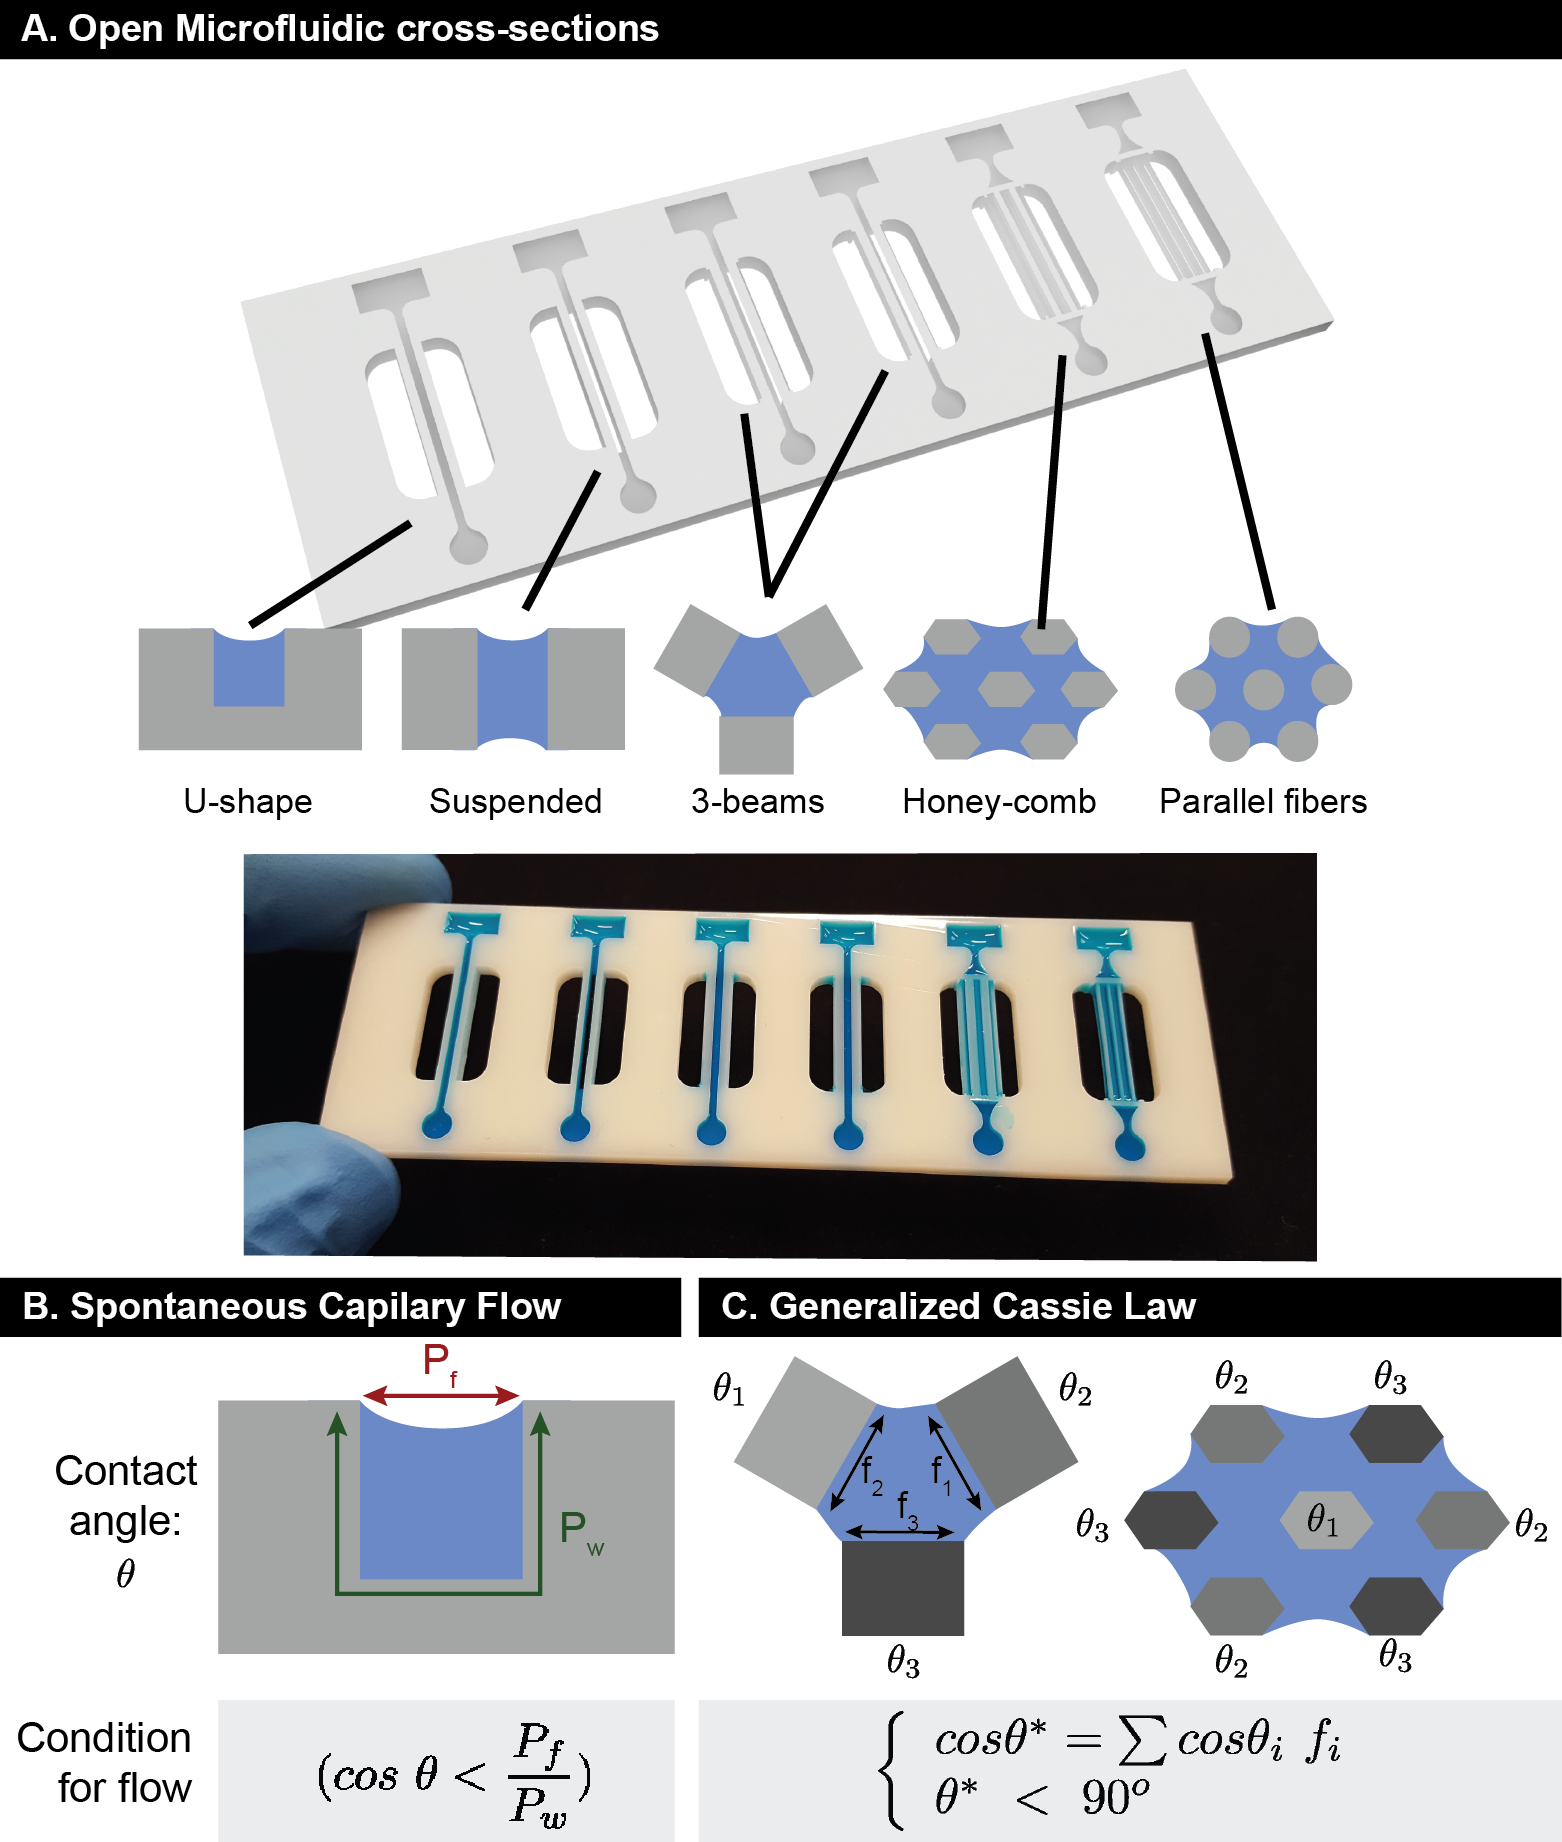
\includegraphics[width=5in]{/OpenFig1.png}
\caption[\textbf{Open microfluidic concepts and generalization of capillary principles}]{\textbf{Open microfluidic concepts and generalization of capillary principles.} (A) 3D printed plate with different cross-sections of open microfluidic channels, including a rectangular groove, a suspended fluid, and suspended beams. (B) Condition for flow in a simple open microfluidic channel in which all the solid faces of the material contacting the fluid have the same contact angle (\texttheta). The perimeter of the cross-section of the channel forming the air-liquid interface is noted $P_f$ and the perimeter of the cross-section of the channel forming the solid-liquid interface is noted $P_w$. (C) Generalization of the Cassie law stating the condition for flow in an open microchannel of any cross-section including materials of different compositions or contact angles.}
\label{figure:OpenFig1}
\end{figure}


\subsection{Open microfluidic enables flow in 3 dimensional systems}
Microfluidic fabrication is a notoriously complex process that has been the subject of intense research. Traditionally microfluidic systems have been designed on planar surfaces such as glass, silicon, or plastic sheets to allow reliable bonding of a cover for the channels \cite{Andersson2003, Rodriguez2003, Iliescu2012}. Open microfluidics inherently alleviates the requirement for complex bonding procedures and the channels can be used immediately after fabrication without the need for subsequent bonding steps. The open nature of the channels also allows for robust and homogeneous treatment of the surfaces, such as plasma treatment, chemical vapor deposition, or spray coating \cite{Casavant2013, Hong2012}

Microfluidics suffers from important reliability and usability barriers. The potential for critical failure of microfluidic channels due to the creation of an air-bubble is a significant limitation towards the use of microsystems in commercial applications. In particular, for systems containing junctures of 2 fluid flows, timing of each flow is critical to prevent air bubble formation. Using open systems, merging any number of flows is robust and independent of synchronization of each flow. Asynchronous fluid flows can be input into the system and air bubbles cannot be created as air can escape from any location along the channel length. 

As no bonding procedure is required, open channels can be created on non-planar and 3-dimensional surfaces in which the fluid starts from a location and can follow a channel imprinted along multiple intersecting planes (Figure \ref{figure:OpenFig2}A,B). When working in 3D geometries gravity can play an important role and create channel failures. Decreasing the SCF condition increases the capillary strength of the open channels and allows fluids to travel robustly in 3-dimensional systems. A precise estimation of the maximum height a fluid can travel in open microfluidic channels can be obtained using the generalized contact angle (equation \ref{equation:OpenEq3}) in the standard height of fluid equation.

\begin{equation}
    \Delta h = \frac{\sum f_{i}\gamma cos \theta}{\rho g a }
    \label{equation:OpenEq3}
\end{equation}


Open microfluidic channels are in particular ideally suited for 3D printing as channels can be designed in any surface of the part, including hidden or upside down surfaces or complex curved surfaces (Figure \ref{figure:OpenFig2}B, C). As every location in the channel is accessible, uncured resin can easily be removed from the channel by rinsing or sonication. This aspect has been utilized to demonstrate the potential geometries and channel configurations presented throughout this document.

When designing open SCF-driven microfluidic channels in 3D space, some precautions must be taken when moving through through acute and right angles. At sharp angles, the geometry of the channel will meet the conditions for Concus-Finn filament formation fluid will leak from the channels into the corners. Fluid leakage can be avoided by rounding corners and locally deepening channels at problem areas, the sharper the angle, the larger radius is needed to prevent leakage and promote SCF in the channel (Figure \ref{figure:OpenFig2}D). 



\begin{figure}[h!] %DONE
\centering
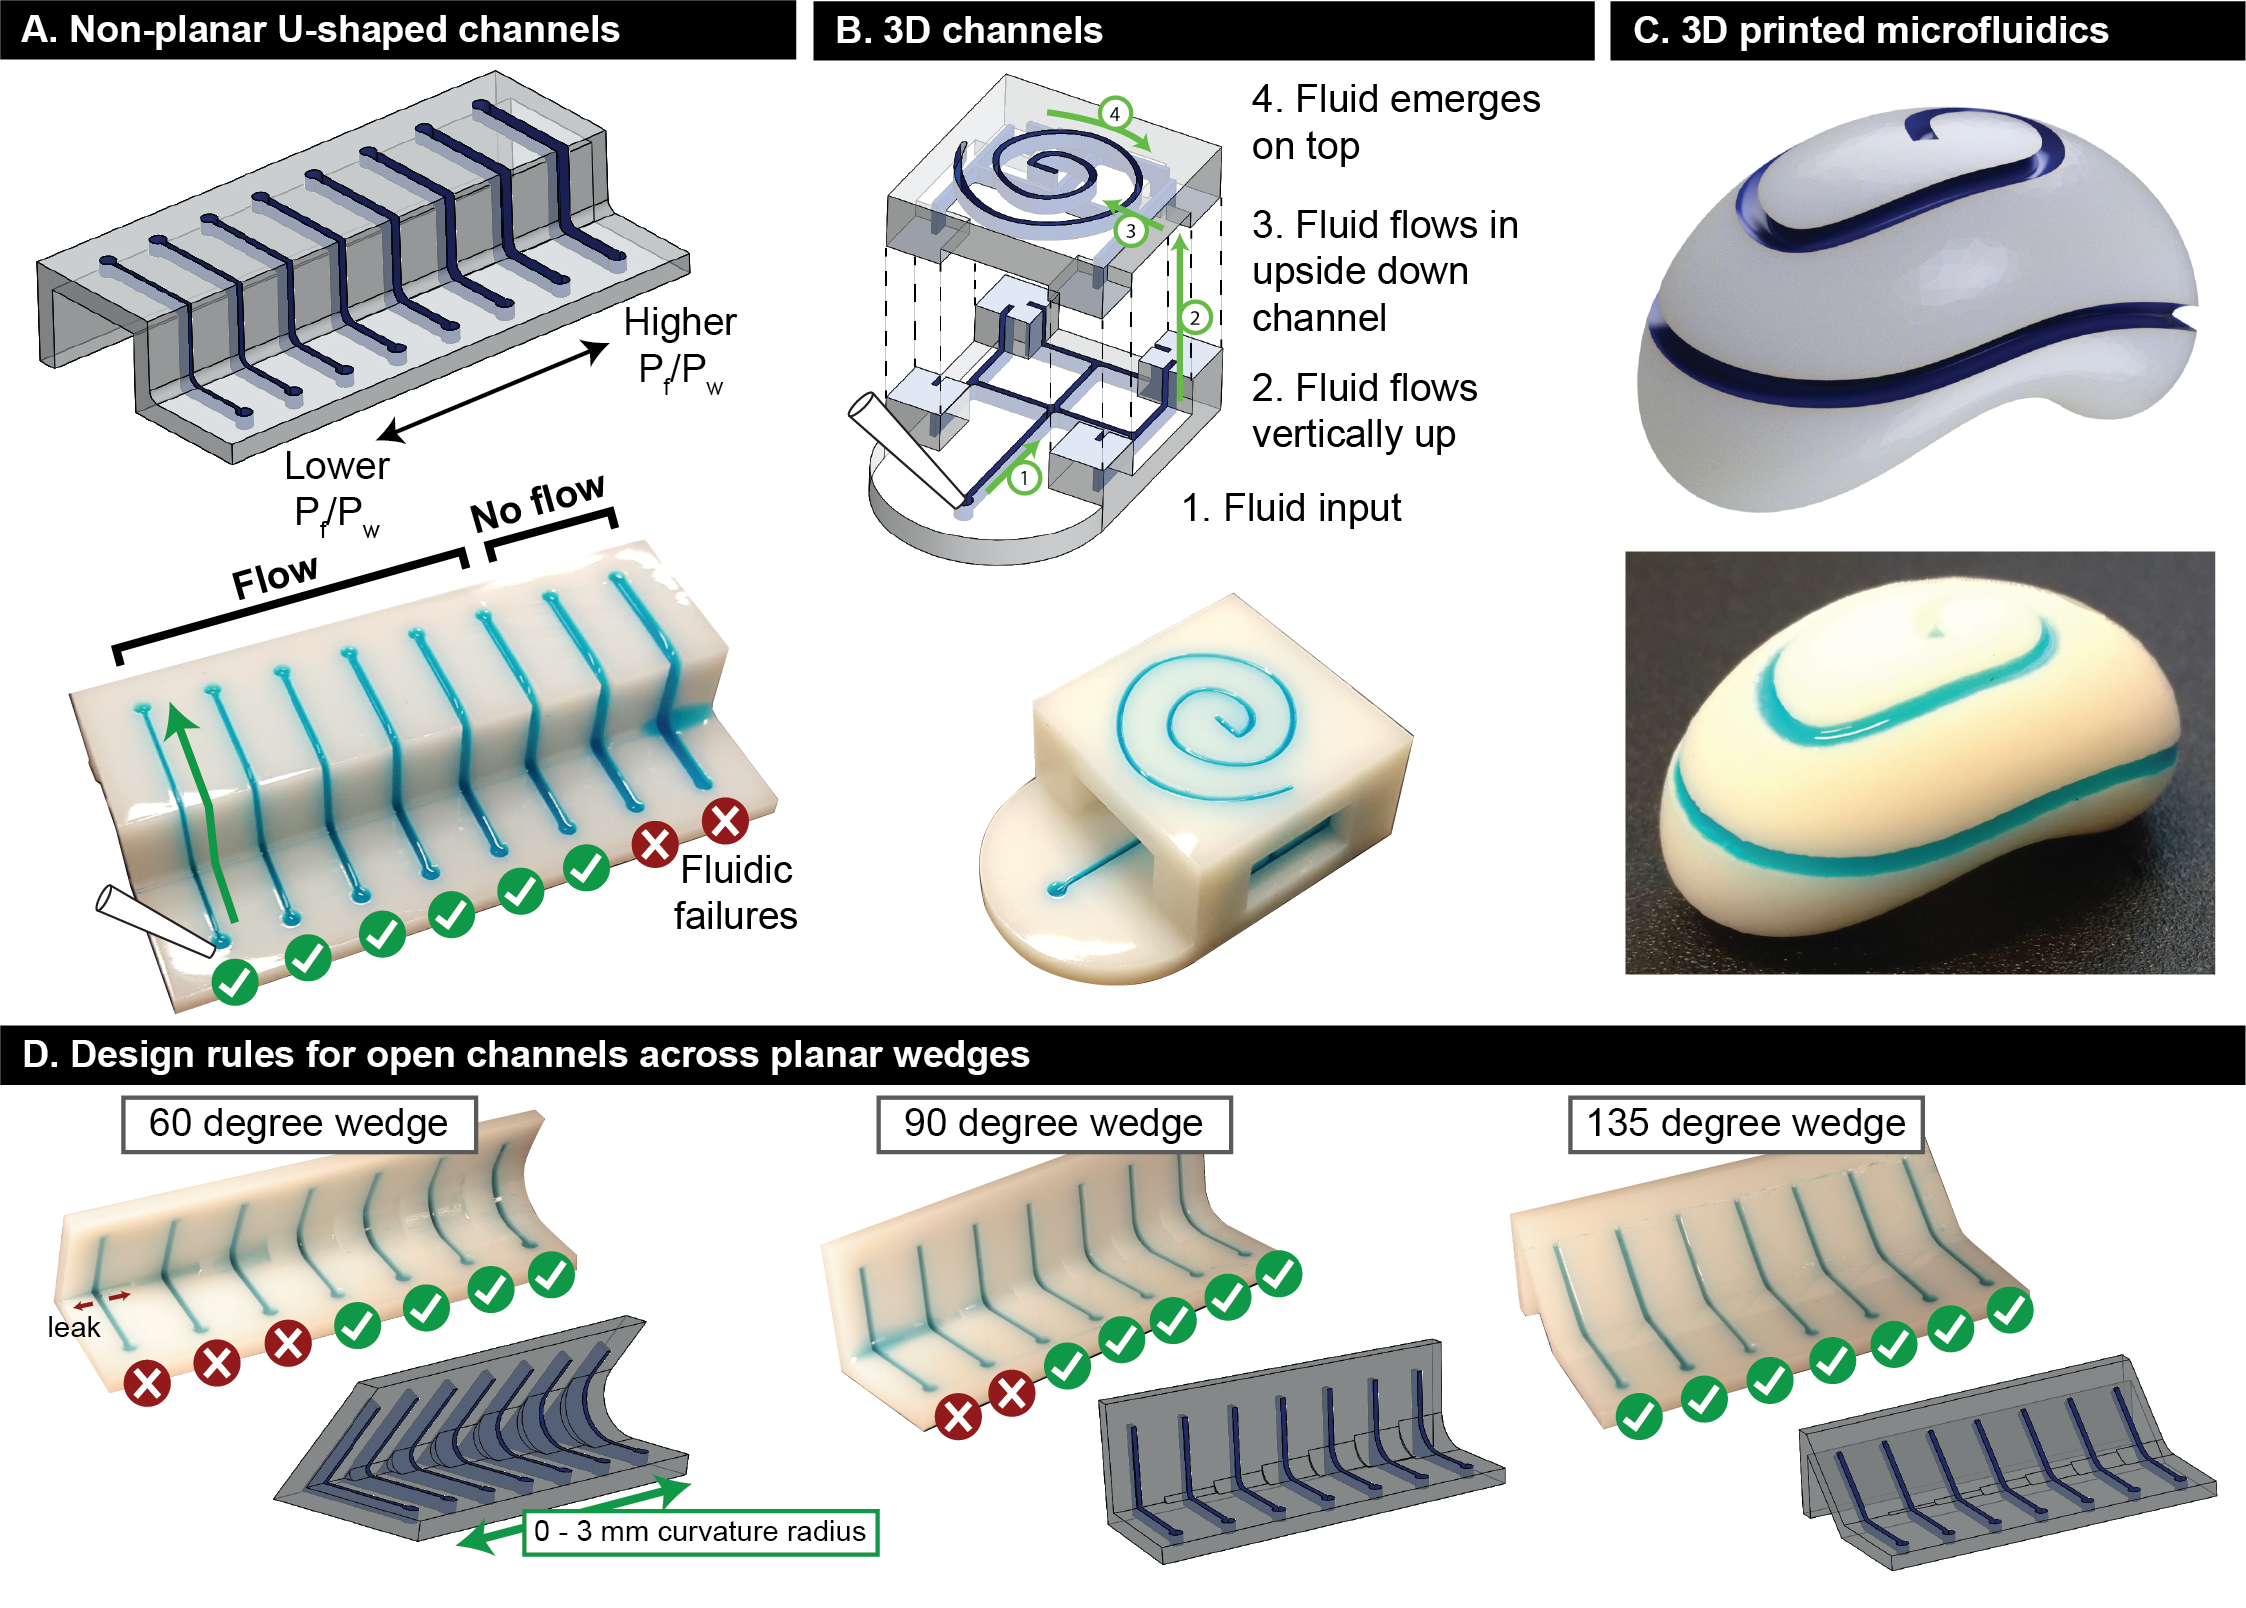
\includegraphics[width=5.5in]{/OpenFig2.png}
\caption[\textbf{Examples of open microfluidic channels}]{\textbf{Examples of open microfluidic channels.} (A) Example of a rectangular cross-section channel flowing up a stepwise channel. A range of width of channels represent different values of $P_f/P_w$. At a certain threshold value, flow is prevented. (B) Example of flow in a complex multifaceted surface designed by SLA printing in which the fluidic path diverges from the horizontal plane. (C) An open microfluidic channel carved into a miniature representation of Cloud Gate or "The Bean" sculpture displayed at the millennium park in Chicago, Illinois. (D) Design considerations for channels running across wedges between 2 planes.}
\label{figure:OpenFig2}
\end{figure}



\subsection{Reconfigurable and modular open microfluidic systems during the operation of the device}

The prototyping power for reconfigurable microfluidic channels has been demonstrated using 3D printed closed microfluidic systems \cite{Bhargava2014}. Open microfluidics, through the use of capillary forces do not have the same requirements for sealing and resisting pressure sources. The ability to function in the open also allows the access of the fluids during the operation of the channel and the creation of systems that are reconfigurable during the operation of the devices. Leveraging these advantages, we have developed a modular, reconfigurable open microfluidic prototyping platform.

The prototyping platform consists of individual blocks with open channels that can be placed on any face of the block. Fluidic components of individual blocks interface with each other with a connector that prevents flow while blocks are separated. The connection consists of a vertical semi-circular open channel that terminates near the bottom of a block (Figure \ref{figure:OpenFig3}A). When filled the pressure is low enough such that the fluid at the end of the channel pins and is held by surface tension. The receptor on the next block in the interface is a tapered pin connected to the open fluidics on its channel. When interfaced, the pin on the lower block breaks the surface tension of the droplet on the upper block and allows flow between blocks. The blocks themselves can be assembled with peg attachment system and can be interfaced with Lego\textregistered\ blocks for use as scaffolding (Figure \ref{figure:OpenFig3}B). The interface at both the fluidic and block level is designed so that individual blocks such as sources and receptacles are easily interchangeable and replaceable and will not result in spilling of fluid allowing for prototyping multi-step or time-based circuits. With this template we can incorporate microfluidic operation onto the blocks, each block has a commonly used microfluidic function like valving, merging fluids, and mixing (Figure \ref{figure:OpenFig3}C). Functional blocks can be assembled into open microfluidic circuits that are not only modular, but reconfigurable during operation. Figure \ref{figure:OpenFig3}D demonstrates a completed open microfluidic circuit and its operation. Fluids can be preloaded in blocks, like reservoir blocks and valved blocks before being initiated. Since it is open, the circuit can be manipulated with a pipette at any place along the fluid path and at any time. Wash cycles in this circuit are achieved by adding preloaded reservoir blocks.


\begin{figure}[h!] %DONE
\centering
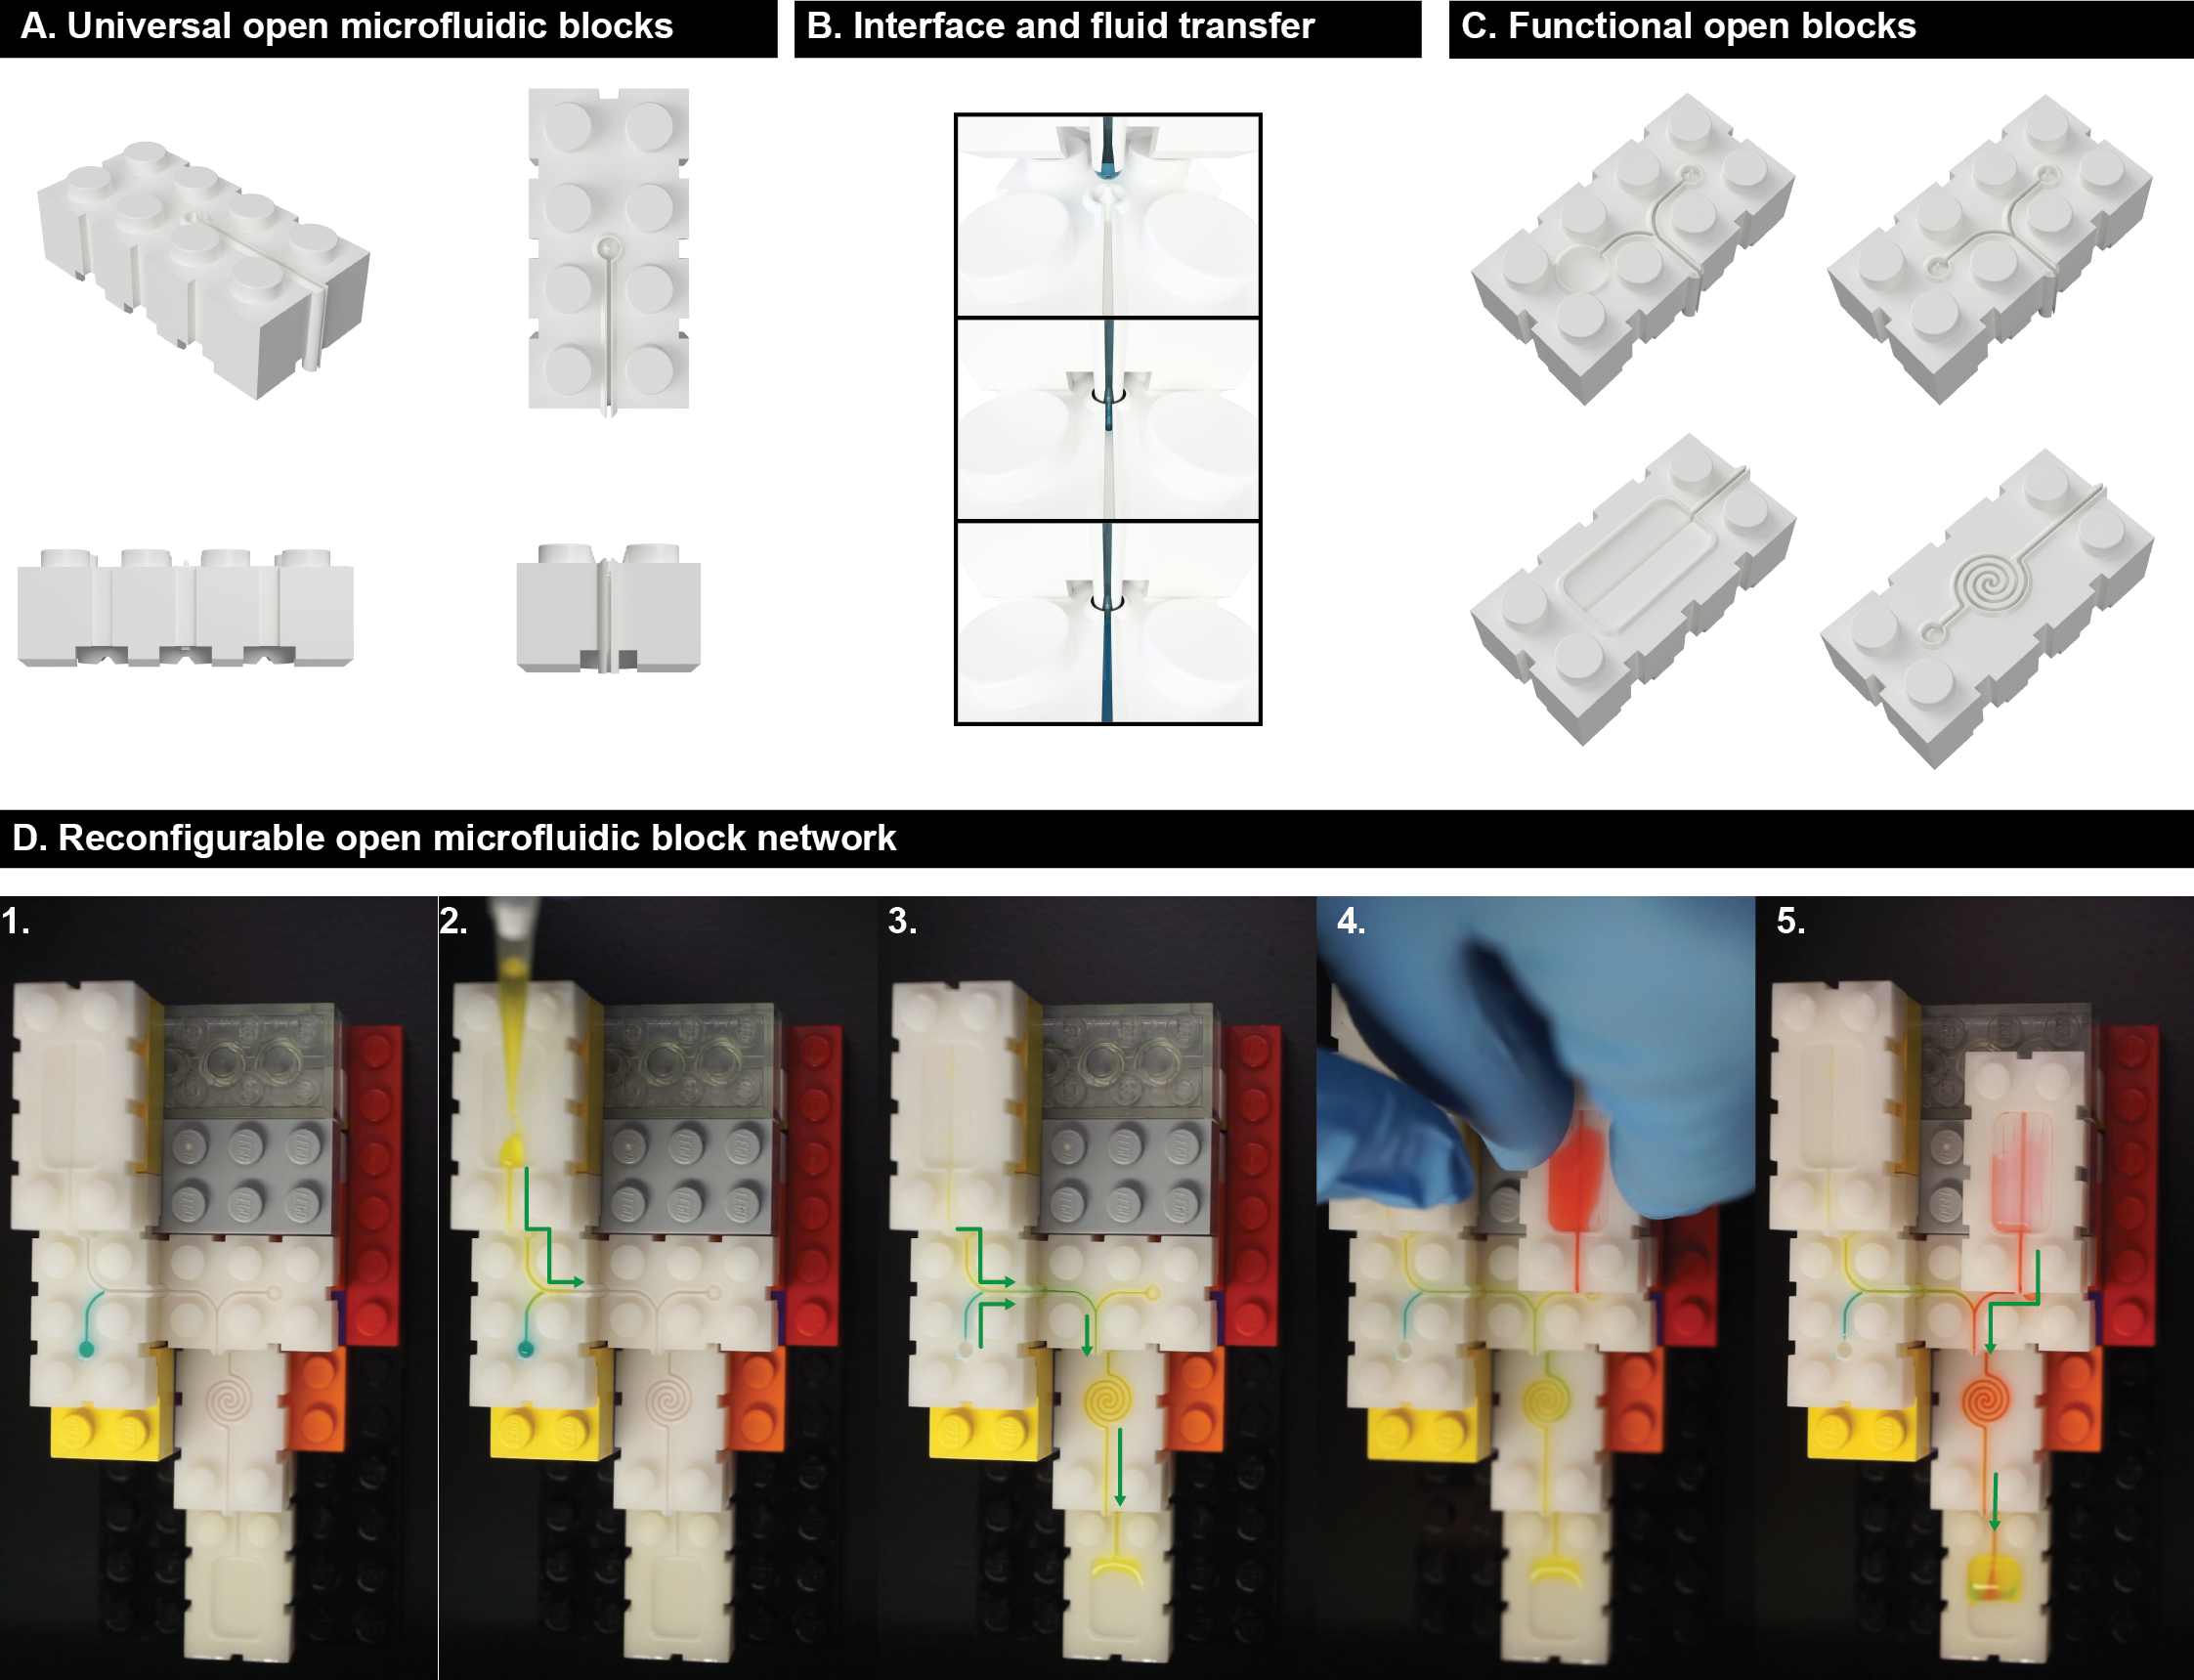
\includegraphics[width=5.75in]{/OpenFig3.png}
\caption[\textbf{A reconfigurable open microfluidic platform}]{\textbf{A reconfigurable open microfluidic platform.} (A) This is example block that has open channel that runs from the center of the top of the block, then across the side, and terminates at the bottom of the structure. The inlet of the open channel consists of a well with a protrusion which interfaces with the outlet of a difference block when the two blocks are placed in phyiscal contact. (B) Several functional blocks used in the construction of open microfluidic networks. Clockwise from the top left: A valving block, a wye-merging block, a mixing block, and a reservoir block. (C) Detailed view of the fluid interface. Two blocks are being brought together with fluid constrained at the outlet of the of the upper block. As they are brought the surface tension holding the fluid together is broken by the pin on the lower block and fluid can be transferred from the upper block to the lower block. (D) Timelapse of a open block network. 1. Fluid is stored in valving block that is part of the network. 2. Fluid is added via pipette through the reservoir and begins flowing through the channel. 3. The added fluid opens the capillary valve and the stored fluid is released. 4. A pre-loaded fluid reservoir block is connected 5. The newly added fluid moves through the network.}
\label{figure:OpenFig3}
\end{figure}
\pagebreak

\subsection{Fluid transfer in open microfluidic designs}

SCF can be used to precisely control fluid volumes in open microfluidic systems based on the geometry of the features alone. When SCF conditions are met in the entire geometry of a channel, the entire channel will be filled when placed in contact with a fluid (so long as there is adequate fluid volume). We are able to exploit this phenomenon to perform sampling from larger fluid reservoirs (Figure \ref{figure:OpenFig4}). We have designed an open microfludic "Ferris wheel" that consists of a hub with a central reservoir and capillary spokes. The inner ends of the spokes are designed to be dipped into the reservoir and pin fluid such that it does not leak and it attached to a capillary channel to draw fluid away from the central reservoir. As the wheel is turned, old spokes leave, and retain the fluid in the capillary and new fluids are able to wick from the central reservoir. This approach could be used to take time dependent samples from reactions of cultures with larger volumes, or even be automated for sample collection over long-term experiments.

We are able to further use capillary action to perform simultaneous sampling from a larger reservoir.Geometries with more favorable SCF conditions are able to pull fluid from geometries with less favorable SCF conditions. We designed a analog-to-digital open microfluidic device capable of extracting precise volumes from a reservoir of fluid (Figure \ref{figure:OpenFig4}B). This devices consists of two parts, a base which acts as a fluid reservoir for the lid, capable of pulling an array of discrete fluid volumes. The base contains a single inlet that is connected by channels to an array of pillars. As fluid is added to the inlet it fills the channels and pillars on the base of the device. The lid contains matching wells each with several fins which fit in pillars on the base and increase the $P_{w}$ to $P_{f}$ ratio of each well. When these two devices are placed in contact, fluid from the base is transferred to the lid of the device, and remains after separating the two layers. This sampling ability is especially useful for applications like digital PCR, where small volumes of fluid from the same source in discrete wells are needed to perform the assay, which is currently performed with active microfluidics.


\begin{figure}[h!] %DONE
\centering
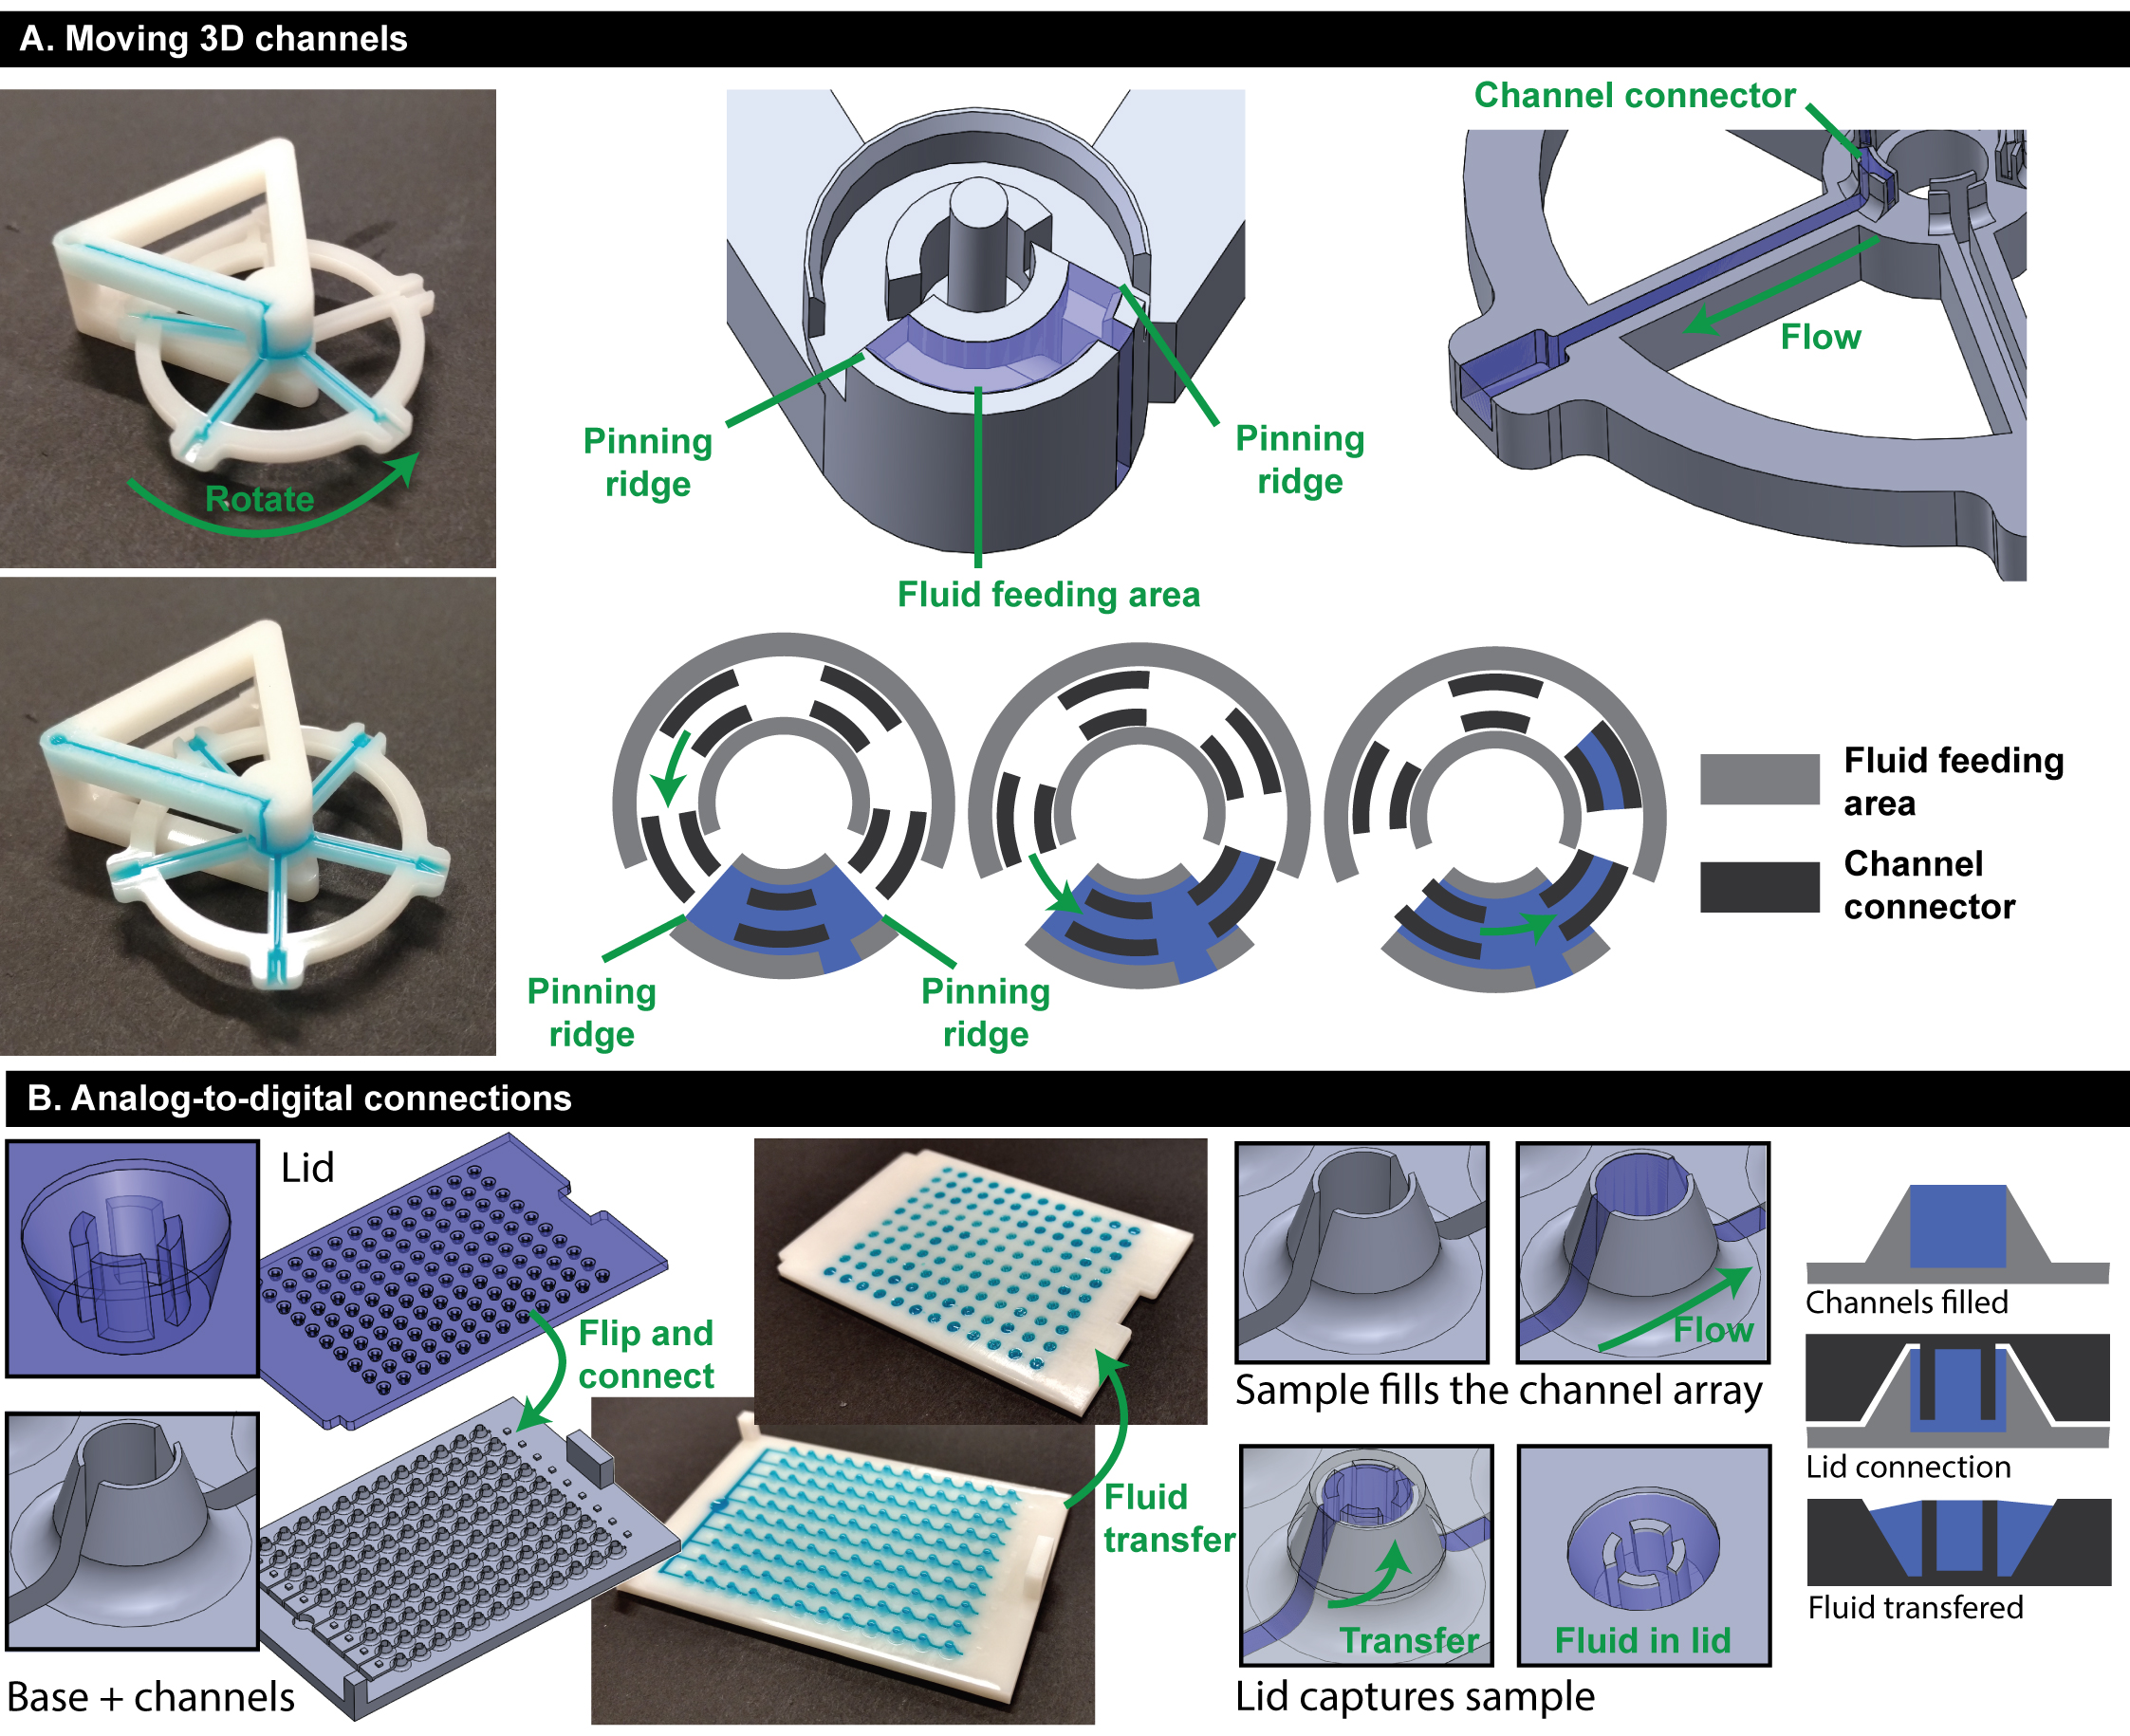
\includegraphics[width=5.75in]{/OpenFig4.jpg}
\caption[\textbf{Fluid sampling with open microfluidics}]{\textbf{Fluid sampling with open microfluidics.} (A) A ferris wheel in which fluid flows into an open channel along the structure of the ferris wheel and connects to a moving wheel. (B) An open microfluidic channel in which continuous flow fills a series of branches in the channel. A digital open microfluidic well array is designed to connect to it and aspirate individual aliquots of fluid. }
\label{figure:OpenFig4}
\end{figure}

\section{Conclusions}
Open microfluidics offers considerable benefits over traditional closed systems. Open microfluidics offers fluid manipulation that is precise and controllable but is accomplished passively, without the need for external pumps. Open microfluidic systems are simple to fabricate since bonding is not required, and amenable to 3D printing allowing rapid dissemination of designs. Fluid flow is spontaneous in open microfluidics and fluid is open channels is accessible throughout the entire channel through pipette or build in sampling. We have demonstrated several capabilities of open microfluidic systems that can be built on to create a range of devices with applications in everything from chemistry to education. 